%-----------------------------------------------------------------------------------------------------------------------------------------------%
%	The MIT License (MIT)
%
%	Copyright (c) 2015 Jan Küster
%
%	Permission is hereby granted, free of charge, to any person obtaining a copy
%	of this software and associated documentation files (the "Software"), to deal
%	in the Software without restriction, including without limitation the rights
%	to use, copy, modify, merge, publish, distribute, sublicense, and/or sell
%	copies of the Software, and to permit persons to whom the Software is
%	furnished to do so, subject to the following conditions:
%
%	THE SOFTWARE IS PROVIDED "AS IS", WITHOUT WARRANTY OF ANY KIND, EXPRESS OR
%	IMPLIED, INCLUDING BUT NOT LIMITED TO THE WARRANTIES OF MERCHANTABILITY,
%	FITNESS FOR A PARTICULAR PURPOSE AND NONINFRINGEMENT. IN NO EVENT SHALL THE
%	AUTHORS OR COPYRIGHT HOLDERS BE LIABLE FOR ANY CLAIM, DAMAGES OR OTHER
%	LIABILITY, WHETHER IN AN ACTION OF CONTRACT, TORT OR OTHERWISE, ARISING FROM,
%	OUT OF OR IN CONNECTION WITH THE SOFTWARE OR THE USE OR OTHER DEALINGS IN
%	THE SOFTWARE.
%
%
%-----------------------------------------------------------------------------------------------------------------------------------------------%


%============================================================================
%
%	DOCUMENT DEFINITION
%
%============================================================================

% Use article class to fully customize the page (do not use use a CV template)
\documentclass[10pt,A4]{article}

\usepackage[utf8]{inputenc}

\usepackage{xifthen}  % provides \isempty test

%----------------------------------------------------------------------------------------
%	FONT
%----------------------------------------------------------------------------------------

% some tex-live fonts - choose your own

%\usepackage[defaultsans]{droidsans}
%\usepackage[default]{comfortaa}
%\usepackage{cmbright}
%\usepackage[default]{raleway}
%\usepackage{fetamont}
\usepackage[default]{gillius}
%\usepackage[light,math]{iwona}
%\usepackage[thin]{roboto}

% set font default
\renewcommand*\familydefault{\sfdefault}
\usepackage[T1]{fontenc}

\usepackage{moresize}     % more font size definitions
\usepackage{fontawesome}
\usepackage{tabularx}

%----------------------------------------------------------------------------------------
%	PAGE LAYOUT  DEFINITIONS
%----------------------------------------------------------------------------------------

%debug page outer frames
%\usepackage{showframe}

%define page styles using geometry
\usepackage[a4paper]{geometry}

% for example, change the margins to 2 inches all round
\geometry{top=1cm, bottom=-.6cm, left=0.4cm, right=1cm}

% less space between header and content
\setlength{\headheight}{-5pt}

%indentation is zero
\setlength{\parindent}{0mm}

%----------------------------------------------------------------------------------------
%	TABLE /ARRAY DEFINITIONS
%----------------------------------------------------------------------------------------

% Layouting tables
\usepackage{multicol}
\usepackage{multirow}

% Extended aligning of tabular cells
\usepackage{array}

\newcolumntype{x}[1]{%
>{\raggedleft\hspace{0pt}}p{#1}}%

%----------------------------------------------------------------------------------------
%	GRAPHICS DEFINITIONS
%----------------------------------------------------------------------------------------

\usepackage{graphicx}

% For floating figures
\usepackage{wrapfig}
\usepackage{float}
%\floatstyle{boxed}
%\restylefloat{figure}

% For drawing graphics
\usepackage{tikz}
\usetikzlibrary{shapes, backgrounds,mindmap, trees}

% Bubble diagrams
\usepackage{smartdiagram}
\smartdiagramset{
    bubble center node font = \footnotesize,
    bubble node font = \footnotesize,
    % specifies the minimum size of the bubble center node
    bubble center node size = 0.5cm,
    %  specifies the minimum size of the bubbles
    bubble node size = 0.9cm,
    % specifies which is the distance among the bubble center node and the other bubbles
    distance center/other bubbles = 0.5cm,
%     % sets the distance from the text to the border of the bubble center node
%     distance text center bubble = 0.5cm,
%     % set center bubble color
%     bubble center node color = pastelblue,
%     % define the list of colors usable in the diagram
%     set color list = {lightgray, materialcyan, orange, green, materialorange, materialteal, materialamber, materialindigo, materialgreen, materiallime},
%     % sets the opacity at which the bubbles are shown
%     bubble fill opacity = 0.6,
%     % sets the opacity at which the bubble text is shown
%     bubble text opacity = 1,
}

%----------------------------------------------------------------------------------------
%	Color DEFINITIONS
%----------------------------------------------------------------------------------------

\usepackage{transparent}
\usepackage{color}

% Accent color
\definecolor{complcol}{RGB}{250,150,10}

% Dark background color
\definecolor{bgcol}{RGB}{110,110,110}

% Light background / Accent color
\definecolor{softcol}{RGB}{225,225,225}
\definecolor{sectcol}{RGB}{0,120,150}

% Other colors
\definecolor{pastelblue}{HTML}{0395DE}

% Package for links, must be the last package used
\usepackage[colorlinks]{hyperref}

%============================================================================%
%
%
%	DEFINITIONS
%
%
%============================================================================%

% Returns minipage width minus two times \fboxsep
% to keep padding included in width calculations
\newcommand{\mpwidth}{\linewidth-\fboxsep-\fboxsep}

%----------------------------------------------------------------------------------------
% 	ARROW GRAPHICS in Tikz
%----------------------------------------------------------------------------------------

% a six pointed arrow poiting to the left
\newcommand{\tzlarrow}{(0,0) -- (0.2,0) -- (0.3,0.2) -- (0.2,0.4) -- (0,0.4) -- (0.1,0.2) -- cycle;}

% include the left arrow into a tikz picture
% param1: fill color
%
\newcommand{\larrow}[1]
{\begin{tikzpicture}[scale=0.58]
	 \filldraw[fill=#1!100,draw=#1!100!black]  \tzlarrow
 \end{tikzpicture}
}

% a six pointed arrow poiting to the right
\newcommand{\tzrarrow}{ (0,0.2) -- (0.1,0) -- (0.3,0) -- (0.2,0.2) -- (0.3,0.4) -- (0.1,0.4) -- cycle;}

% include the right arrow into a tikz picture
% param1: fill color
%
\newcommand{\rarrow}
{
\begin{tikzpicture}[scale=0.7]
	\filldraw[fill=sectcol!100,draw=sectcol!100!black] \tzrarrow
 \end{tikzpicture}
}

%----------------------------------------------------------------------------------------
%	custom sections
%----------------------------------------------------------------------------------------

% create a coloured box with arrow and title as cv section headline
% param 1: section title
%
\newcommand{\cvsection}[1]{
  \colorbox{sectcol}{\mystrut \makebox[1\mpwidth][l]{
  \larrow{bgcol} \hspace{-8pt} \larrow{bgcol} \hspace{-8pt} \larrow{bgcol} \textbf{\textcolor{white}{\uppercase{#1}}}\hspace{4pt}
  }}\\
}

% create a coloured arrow with title as cv meta section section
% param 1: meta section title
%
\newenvironment{metasection}[1] {
	\vspace{6pt}
	\begin{center}
		\textcolor{white}{\large{\uppercase{#1}}}\\
	\normalsize
	\parbox{0.7\mpwidth}{\textcolor{white}	\hrule}
}{\end{center}}

%----------------------------------------------------------------------------------------
%	 CV ENTRIES: cvposition, cventry, cvevent (the original one)
%----------------------------------------------------------------------------------------

% Company/position heading command
% arg1: dates
% arg2: position
% arg3: company
\newcommand{\cvposition}[3]{
  \vspace{8pt}
  \begin{tabular*}{1\mpwidth}{p{0.45\mpwidth}  x{0.52\mpwidth}}
    \textcolor{black}{\textbf{#2}} & \textcolor{complcol}{#3}, \textcolor{bgcol}{#1}
  \end{tabular*}
  \textcolor{softcol}{\hrule}\vspace{6pt}
}

\newcommand{\cventry}[1]{
  \vspace{6pt}
%   \par
  \begin{minipage}[t]{0.04\mpwidth}
    \hspace{3pt}\larrow{softcol}
  \end{minipage}
  \begin{minipage}[t]{0.97\mpwidth}
    #1
  \end{minipage}
  \par
}

% creates a stretched box as cv entry headline followed by two paragraphs about
% the work you did
% param 1:	event time i.e. 2014 or 2011-2014 etc.
% param 2:	event name (what did you do?)
% param 3:	institution (where did you work / study)
% param 4:	what was your position
% param 5:	some words about your contributions
%
\newcommand{\cvevent}[5]
{
\vspace{8pt}
	\begin{tabular*}{1\mpwidth}{p{0.55\mpwidth}  x{0.42\mpwidth}}
 	\textcolor{black}{\textbf{#2}} & \textcolor{complcol}{#3}, \textcolor{bgcol}{#1}

	\end{tabular*}
\vspace{-12pt}
\textcolor{softcol}{\hrule}
\vspace{6pt}
	\begin{tabular*}{0.5\mpwidth}{p{\mpwidth}}
\larrow{softcol}  #4\\[3pt]
\larrow{softcol}  #5\\[6pt]
	\end{tabular*}
}

% creates a stretched box as
\newcommand{\cveventmeta}[2]
{
	\mbox{\mystrut \hspace{87pt}\textit{#1}}\\
	#2
}

%----------------------------------------------------------------------------------------
% CUSTOM STRUT FOR EMPTY BOXES
%----------------------------------------- -----------------------------------------------
\newcommand{\mystrut}{\rule[-.3\baselineskip]{0pt}{\baselineskip}}

%----------------------------------------------------------------------------------------
% CUSTOM LOREM IPSUM
%----------------------------------------------------------------------------------------
\newcommand{\lorem}
{Lorem ipsum dolor sit amet, consectetur adipiscing elit. Donec a diam lectus.}

% use to vertically center content
% credits to: http://tex.stackexchange.com/questions/7219/how-to-vertically-center-two-images-next-to-each-other
\newcommand{\vcenteredinclude}[1]{\begingroup
\setbox0=\hbox{\includegraphics{#1}}%
\parbox{\wd0}{\box0}\endgroup}

% use to vertically center content
% credits to: http://tex.stackexchange.com/questions/7219/how-to-vertically-center-two-images-next-to-each-other
\newcommand*{\vcenteredhbox}[1]{\begingroup
\setbox0=\hbox{#1}\parbox{\wd0}{\box0}\endgroup}

%----------------------------------------------------------------------------------------
%	ICON MACROS
%----------------------------------------------------------------------------------------

% args: (iconName, boxSize, color)
\newcommand{\icon}[3]{%	                        %icon shortcut
    \vcenteredhbox{\makebox(#2, #2){\textcolor{#3}{\csname fa#1\endcsname}}}%
}

% args: (iconName, boxSize, text, color)
\newcommand{\icontext}[4]{ 						%icon with text shortcut
    \vcenteredhbox{\icon{#1}{#2}{#4}} \vcenteredhbox{\textcolor{#4}{#3}}
}

% args: (iconName, boxSize, text, url, textColor)
\newcommand{\iconhref}[5]{ 						%icon with website url
    \vcenteredhbox{\icon{#1}{#2}{#5}} \href{#4}{\textcolor{#5}{#3}}
}

% args: (iconName, boxSize, text, mailto, color)
\newcommand{\iconemail}[5]{ 					%icon with email link
    \vcenteredhbox{\icon{#1}{#2}{#5}} \href{mailto:#4}{\textcolor{#5}{#3}}
}

%============================================================================
%
%	DOCUMENT CONTENT
%
%============================================================================

\begin{document}
\fcolorbox{white}{white}{\begin{minipage}[c][0.95\textheight][t]{0.69\linewidth}

%---------------------------------------------------------------------------------------
%	TITLE HEADLINE
%----------------------------------------------------------------------------------------

\vspace{-3pt}
\colorbox{bgcol}{\makebox[\mpwidth][c]{
  \hspace{46pt}\HUGE{\textcolor{white}{\uppercase{Gerard Bosch}} }
  \textcolor{sectcol}{\rule[-1mm]{1mm}{0.9cm}}
  \parbox[b]{5cm}{
    \large{\textcolor{white}{{Software Engineer}}} \\
    \large{\textcolor{white}{{Craftsman}}}
  }
}}

%----------------------------------------------------------------------------------------
%	HEADER IMAGE
%----------------------------------------------------------------------------------------

%\includegraphics[trim= 350 150 0 200, clip ,width=\linewidth]{}  %trimming relative to image size
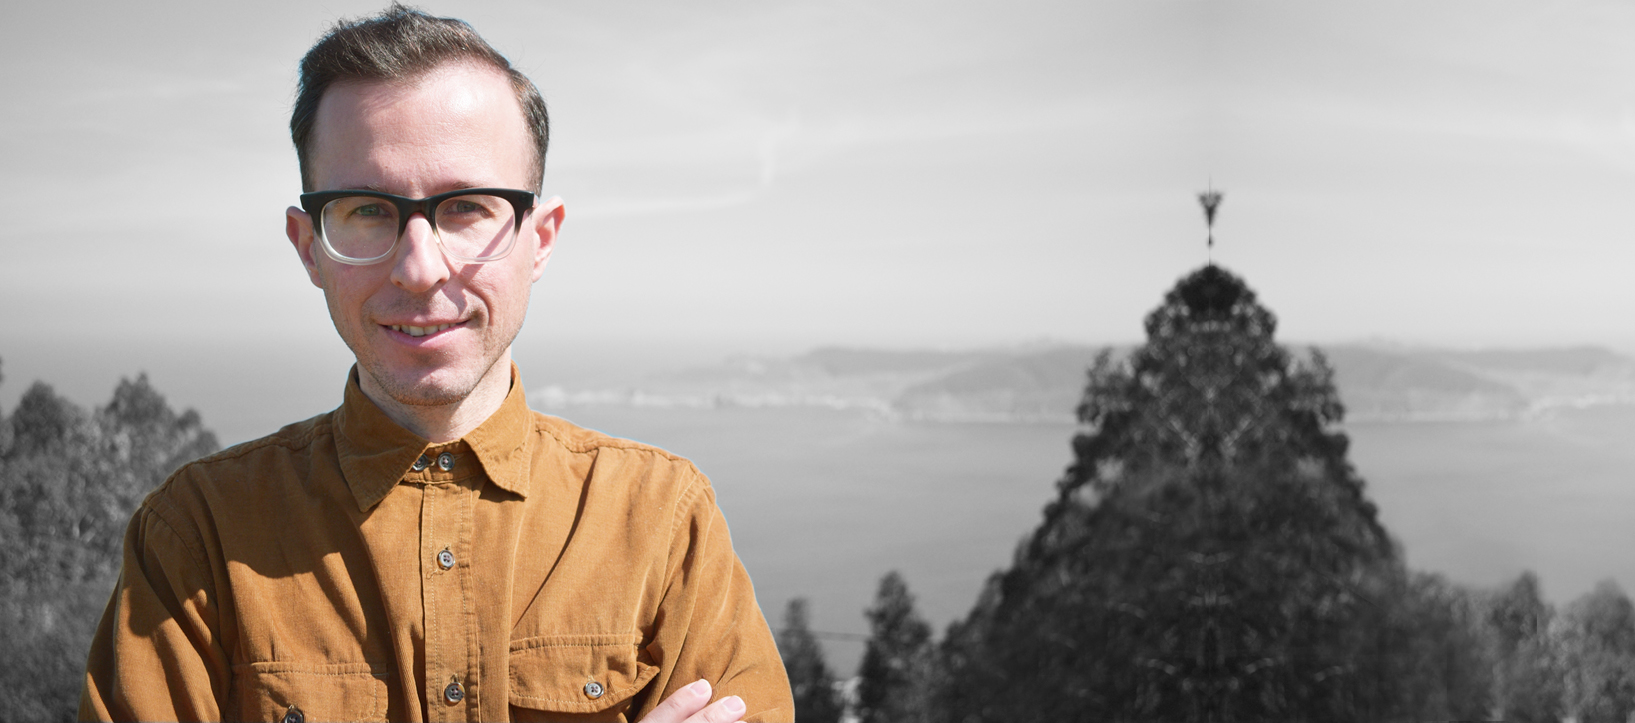
\includegraphics[clip, width=\linewidth]{pic-header.jpg}

%---------------------------------------------------------------------------------------
%	INTRODUCTION
%----------------------------------------------------------------------------------------
\transparent{0.85}%
\vspace{-130pt}
\hspace{0.4\linewidth}
\colorbox{bgcol}{
	\parbox{0.5\linewidth}{
		\transparent{1}%
		\begin{center}
		\larrow{sectcol}\textcolor{white}{
		  Enthusiast about Functional Programming, software engineering/craftsmanship, clean code, architectural/design
		  patterns and programming languages theory.
		}
		\end{center}
	}
}
\vspace{60pt}

%============================================================================%
%
%	CV SECTIONS AND EVENTS (MAIN CONTENT)
%
%============================================================================%

%---------------------------------------------------------------------------------------
%	SUMMARY
%----------------------------------------------------------------------------------------
\cvsection{Summary}

[ \emph{Read the full detailed CV at} \href{https://github.com/gerardbosch/cv}{https://gerardbosch.github.io/cv} ] \\[-2pt]

My background is mostly about designing and implementing backend systems. I have good analysis skills and can break down requirements well and transform that into code. Really concerned about the code itself, its readability and conciseness.

\vspace{12pt}

%---------------------------------------------------------------------------------------
%	EXPERIENCE
%----------------------------------------------------------------------------------------
\cvsection{Experience}

% Original cvevent example
%\cvevent{2020 - now}{}{}{}{}
%\textcolor{softcol}{\hrule}

% New custom commands below :)

\cvposition{2016 - now}{Senior Software Engineer}{GFT IT Consulting}

~~PROJECT HIGHLIGHTS (most relevant ones):

\cventry{
  \textit{Banc Sabadell}: \textbf{Middleware Architecture} (2020\ldots) -- Redefine from scratch a whole new framework and development environment based on MsA, Spring Boot, API-First, Event Driven, DDD, Hexagonal and so forth -- \textbf{Role}: Software Engineer.
}

\cventry{
  \textit{Banc Sabadell}: \textbf{PSD2 \& APIfication} (2018--2020) -- Design \& implement the APIs for the European regulatory PSD2 project, leading the first approach to API exposition for the Banc. Definine and implement architectural components for the MsA where I was established as the technical lead for the dev team -- \textbf{Role}: Tech Lead.
}

\cventry{
  \textit{Bankinter}: \textbf{Microservice Architecture} (2017) -- Development of an architecture based on MsA and Spring, providing the pre-configured components: from security, tracing, audit, error handling to cryptography; enabling developers to easily get started.
}

% Example using itemize (more vertical space)
% \cvevent{2016 - now}{Senior Software Engineer}{GFT IT Consulting}
%   {\textbf{PROJECT HIGHLIGHTS} (most relevant only)
%   \begin{itemize}
%      \item \textit{Banc Sabadell}: \textbf{Middleware Architecture} (2020\ldots) -- Redefine from scratch a whole new framework and development environment based on MsA, Spring Boot, API-First, Event Driven, DDD, Hexagonal and so forth -- \textbf{Role}: Software Engineer.
%
%      \item \textit{Banc Sabadell}: \textbf{PSD2 \& APIfication} (2018--2020) -- Design \& implement the APIs for the european regulatory PSD2 project, leading the first approach to API exposition for the Banc. Definine and implement architectural components for the MsA where
%      I was established as the technical lead for the dev team -- \textbf{Role}: Tech Lead.
%
%      \item \textit{Bankinter}: \textbf{Microservice Architecture} (2017)
%      Worked in the development of an architecture for Bankinter based on MSA (Micro Services Architecture) with Java 8 and Spring Boot/Cloud. The Architecture provided the preconfigured components: from security, logging, audit,... to cryptography to allow developers to easily get started implementing small micro-services with not much Spring background required -- \textbf{Role}: Software Engineer.
%   \end{itemize}
%   }

\cvposition{2014--2016}{Software Engineer}{ICG Software}
\cventry{Senior developer in charge of mobile solutions for business domains.}\vspace{-8pt}
\cventry{Architecting mobile applications for Android and Windows Phone platforms.}

\cvposition{2011--2013}{Researcher/developer}{AI Research Institute IIIA-CSIC}
~~Spanish National Research Council. Innpacto-2011 (Spanish Science and Innovation Ministry),\par\vspace{2pt}
~~\emph{NEWMATICA: Intelligent and Energy Efficient Advanced System for Vacuum Waste Collection}.

\cventry{Research on artificial intelligence algorithms and machine learning.}\vspace{-8pt}
\cventry{
  Implement \emph{Approximate Dynamic Programming} (Reinforcement Learning) algorithms in order to optimize operational plans of waste collecting plants.
}
\cventry{Implement a waste collecting simulator, run simulations, collect data/process results.}


%---------------------------------------------------------------------------------------
%	EDUCATION SECTION
%--------------------------------------------------------------------------------------
\cvsection{Education}

\cvposition{2011}{M.Sc. Open Source Software Eng.}{University of Lleida}\vspace{-2pt}
\cventry{Master Thesis: \emph{Setting up and deployment of Sauron system for DNS system management at University of Lleida.}}
\cventry{Mobility program internship in \emph{VIA UC}, Denmark.}

~~\emph{To see more, view the CV version.}

% \cvposition{2010}{Bachelor Computer Science}{University of Lleida}\vspace{-2pt}
% \cventry{Bachelor Thesis: \emph{Implementation of Golay codes in Sage Math.}}


\end{minipage}}%
\fcolorbox{white}{sectcol}{\begin{minipage}[c][0.95\textheight][t]{0.33\linewidth}


%----------------------------------------------------------------------------------------
%	SIDE BAR
%----------------------------------------------------------------------------------------

\begin{metasection}{Contact}

	\icontext{MapMarker}{12}{Barcelona, Spain}{white}\\[5pt]
	\icontext{MobilePhone}{12}{+34 680 271 551}{white}\\[5pt]
	\iconemail{Envelope}{12}{gerard.bosch@gmail.com}{gerard.bosch@gmail.com}{white} \\[5pt]
	%\iconhref{MousePointer}{12}{Webpage}{Webpage}{white} \\[5pt]
	\iconhref{Github}{12}{https://github.com/gerardbosch}{https://github.com/gerardbosch}{white} \\[5pt]
	\iconhref{StackOverflow}{12}{https://stackoverflow.com/gerard-bosch}{https://stackoverflow.com/gerard-bosch}{white} \\[5pt]
	%\iconhref{Twitter}{12}{@user}{https://twitter.com/user}{white} \\[5pt]

\end{metasection}

\vspace{-0.3cm}
\begin{metasection}{Programming Lang}\color{white}
\vspace{5pt}
\begin{tabular}{rl}

Java 15 &
\icon{Star}{12}{complcol}\icon{Star}{12}{complcol}\icon{Star}{12}{complcol}\icon{Star}{12}{complcol}\icon{Star}{12}{complcol} \\[5pt]

Scala &
\icon{Star}{12}{complcol}\icon{Star}{12}{complcol}\icon{Star}{12}{complcol}\icon{Star}{12}{complcol}\icon{Star}{12}{white} \\[5pt]

Kotlin &
\icon{Star}{12}{complcol}\icon{Star}{12}{complcol}\icon{Star}{12}{complcol}\icon{Star}{12}{white}\icon{Star}{12}{white} \\[5pt]

Bash &
\icon{Star}{12}{complcol}\icon{Star}{12}{complcol}\icon{Star}{12}{complcol}\icon{Star}{12}{complcol}\icon{Star}{12}{white} \\[5pt]

Haskell &
\icon{Star}{12}{complcol}\icon{Star}{12}{complcol}\icon{Star}{12}{complcol}\icon{Star}{12}{white}\icon{Star}{12}{white} \\[5pt]

Python &
\icon{Star}{12}{complcol}\icon{Star}{12}{complcol}\icon{Star}{12}{complcol}\icon{Star}{12}{white}\icon{Star}{12}{white} \\[5pt]

Perl &
\icon{Star}{12}{complcol}\icon{Star}{12}{white}\icon{Star}{12}{white}\icon{Star}{12}{white}\icon{Star}{12}{white}

\end{tabular}
\end{metasection}


\vspace{-0.3cm}
\begin{metasection}{Technologies}

\icontext{Code}{12}{Spring Boot}{white}
\icontext{Key}{12}{oAuth}{white} \\[5pt]

\icontext{Cubes}{12}{Maven}{white}
\icontext{Cubes}{12}{Gradle}{white}
\icontext{Cubes}{12}{SBT}{white} \\[5pt]


\icontext{Code}{12}{Vavr}{white}
\icontext{PuzzlePiece}{12}{API First \& OpenAPI 3}{white} \\[5pt]
\icontext{LifeSaver}{12}{JGitVer}{white}
\icontext{Terminal}{12}{Docker}{white}

\end{metasection}


\vspace{-0.3cm}
\begin{metasection}{Tools}

\icontext{Code}{12}{IntelliJ}{white} \icontext{CodeFork}{12}{Git (sure!)}{white}
\icontext{Terminal}{12}{ZSH}{white}

\end{metasection}

% \begin{metasection}{Activities}
%
% \textcolor{white}{\LARGE{\icon{Gamepad}{24}{white} \icon{Headphones}{24}{white}  \icon{Bicycle}{24}{white}}}
% \end{metasection}
%
% \begin{metasection}{Operating Systems}
%
% \textcolor{white}{\LARGE{\icon{Linux}{24}{white} \icon{Apple}{24}{white}  \icon{Windows}{24}{white}}}
%
% \end{metasection}


%---------------------------------------------------------------------------------------
%	Knowledge Areas
%----------------------------------------------------------------------------------------

\vspace{-0.3cm}
\begin{metasection}{In graphics...}
\begin{center}

\smartdiagramset{
    bubble center node font = \footnotesize,
    bubble node font = \footnotesize,
    % specifies the minimum size of the bubble center node
    bubble center node size = 0.1cm,
    %  specifies the minimum size of the bubbles
    bubble node size = 0.9cm,
    % specifies which is the distance among the bubble center node and the other bubbles
    distance center/other bubbles = 0.5cm,
%     % sets the distance from the text to the border of the bubble center node
%     distance text center bubble = 0.5cm,
%     % set center bubble color
    bubble center node color = pastelblue,
%     % define the list of colors usable in the diagram
%     set color list = {lightgray, materialcyan, orange, green, materialorange, materialteal, materialamber, materialindigo, materialgreen, materiallime},
%     % sets the opacity at which the bubbles are shown
%     bubble fill opacity = 0.6,
%     % sets the opacity at which the bubble text is shown
%     bubble text opacity = 1,
}
\smartdiagram[bubble diagram]{
    Knowledge \\ Areas,
    \normalsize{\textbf{Functional}} \\ \normalsize{\textbf{Programming}},
    DevOps,
    Reactive \\ Programming,
    \normalsize{\textbf{API design}} \\ \normalsize{\textbf{\& Tooling}},
    \normalsize{\textbf{~~Design~~}} \\ \normalsize{\textbf{patterns}},
    \textbf{Architectural} \\ \textbf{patterns},
    API\\ security
}

\smartdiagramset{
    bubble center node font = \footnotesize,
    bubble node font = \footnotesize,
    % specifies the minimum size of the bubble center node
    bubble center node size = 0.1cm,
    %  specifies the minimum size of the bubbles
    bubble node size = 0.9cm,
    % specifies which is the distance among the bubble center node and the other bubbles
    distance center/other bubbles = 0.5cm,
%     % sets the distance from the text to the border of the bubble center node
%     distance text center bubble = 0.5cm,
%     % set center bubble color
    bubble center node color = orange,
%     % define the list of colors usable in the diagram
%     set color list = {lightgray, materialcyan, orange, green, materialorange, materialteal, materialamber, materialindigo, materialgreen, materiallime},
%     % sets the opacity at which the bubbles are shown
%     bubble fill opacity = 0.6,
%     % sets the opacity at which the bubble text is shown
%     bubble text opacity = 1,
}
\smartdiagram[bubble diagram]{
    \normalsize{Interest} \\ \normalsize{Areas},
    \textbf{~~~~DLTs \&~~~~} \\ \textbf{Blockchain},
    \textbf{Functional} \\ \textbf{Programming},
    \textbf{Artificial} \\ \textbf{Intelligence},
    \textbf{Big/Fast Data} \\ \textbf{\& Streaming}
}

\end{center}
\end{metasection}


%%%%%%%%%%%%%%%%%%%%%%%%%%%%%%%%%
\end{minipage}}    % end side bar
%%%%%%%%%%%%%%%%%%%%%%%%%%%%%%%%%


%-------------------------------------------------------------------------------------------------
%	ARTIFICIAL FOOTER (fancy footer cannot exceed linewidth)
%--------------------------------------------------------------------------------------------------

\null
\vspace*{\fill}
\hspace{-0.25\linewidth}\colorbox{bgcol}{\makebox[1.5\linewidth][c]{
  \mystrut \small \textcolor{white}{
    \LaTeX~source of this \textit{résumé} is available at
    \iconhref{Github}{12}{https://github.com/gerardbosch/resume}{https://github.com/gerardbosch/resume}{white}
  }
}}

%============================================================================%
%
%	DOCUMENT END
%
%============================================================================%
\end{document}
